\documentclass[a4paper, 14pt]{extarticle}

% Поля
%----------------------
\usepackage{geometry}
\geometry{a4paper,left=2cm,right=1cm,
    top=2cm,bottom=2cm,bindingoffset=0cm}
%----------------------

% Russian-specific packages
%----------------------
\usepackage[T2A]{fontenc}
\usepackage[utf8]{inputenc}
\usepackage[english, main=russian]{babel}
%----------------------

\usepackage{textcomp}

% Красная строка
%----------------------
\usepackage{indentfirst}
%----------------------

% Graphics
%----------------------
\usepackage{graphicx}
\graphicspath{ {./images} }
\usepackage{wrapfig}
%----------------------

% Import minted
%----------------------
\usepackage{minted}
%----------------------

\linespread{1.3}
\sloppy
\clubpenalty=10000
\widowpenalty=10000

\begin{document}

%--------------------------------------
%			ТИТУЛЬНЫЙ ЛИСТ
%--------------------------------------
\begin{titlepage}
\thispagestyle{empty}
\newpage


%Шапка титульного листа
%--------------------------------------
\vspace*{-60pt}
\hspace{-65pt}
\begin{minipage}{0.3\textwidth}
\hspace*{-20pt}\centering

\includegraphics[width=\textwidth]{emblem}
\end{minipage}
\begin{minipage}{0.67\textwidth}\small \textbf{
\vspace*{-0.7ex}
\hspace*{-6pt}\centerline{Министерство науки и высшего образования Российской Федерации}
\vspace*{-0.7ex}
\centerline{Федеральное государственное бюджетное образовательное учреждение }
\vspace*{-0.7ex}
\centerline{высшего образования}
\vspace*{-0.7ex}
\centerline{<<Московский государственный технический университет}
\vspace*{-0.7ex}
\centerline{имени Н.Э. Баумана}
\vspace*{-0.7ex}
\centerline{(национальный исследовательский университет)>>}
\vspace*{-0.7ex}
\centerline{(МГТУ им. Н.Э. Баумана)}}
\end{minipage}
%--------------------------------------

%Полосы
%--------------------------------------
\vspace{-25pt}
\hspace{-35pt}\rule{\textwidth}{2.3pt}

\vspace*{-20.3pt}
\hspace{-35pt}\rule{\textwidth}{0.4pt}
%--------------------------------------

\vspace{1.5ex}
\hspace{-35pt} \noindent \small ФАКУЛЬТЕТ\hspace{80pt} <<Информатика и системы управления>>

\vspace*{-16pt}
\hspace{47pt}\rule{0.83\textwidth}{0.4pt}

\vspace{0.5ex}
\hspace{-35pt} \noindent \small КАФЕДРА\hspace{50pt} <<Теоретическая информатика и компьютерные технологии>>

\vspace*{-16pt}
\hspace{30pt}\rule{0.866\textwidth}{0.4pt}
  
\vspace{11em}

\begin{center}
\Large {\bf Лабораторная работа № 5} \\ 
\large {\bf по курсу <<Языки и методы программирования>>} \\
\large <<Монады в языке Java>> \\
\large Вариант 34
\end{center}\normalsize

\vspace{8em}


\begin{flushright}
  {Студент группы ИУ9-22Б Павлов И. П. \hspace*{15pt}\\ 
  \vspace{2ex}
  Преподаватель Посевин Д. П.\hspace*{15pt}}
\end{flushright}

\bigskip

\vfill
 

\begin{center}
\textsl{Москва 2023}
\end{center}
\end{titlepage}
%--------------------------------------
%		КОНЕЦ ТИТУЛЬНОГО ЛИСТА
%--------------------------------------

\newpage
\section{Цель работы}
Приобретение навыков использования монад Optional и Stream в программах на языке
Java.

\section{Условие}
Во время выполнения лабораторной работы требуется разработать на языке Java один
из классов, перечисленных в таблице, которая приведена ниже.

В каждом классе нужно реализовать по крайней мере два метода: первый метод
должен возвращать Stream, а второй – Optional. Операции, выполняемые каждым методом,
указаны в вариантах задания.

Реализовать множество целых чисел с операциями:

1. порождение потока попарных произведений элементов множества;

2. поиск числa x такого, что любой элемент множества находится в диапазоне (-x, x).

Проверить работу первой операции нужно путём ранжирования произведений на три
группы: отрицательные, нулевые и положительные.

\section{Реализация основного класса}
{\scriptsize
\begin{minted}{java}
public class Main {

    public static void main(String[] args) {
        Numbers myNumbers = new Numbers();

        // Добавим в множество несколько чисел
        myNumbers.addNumber(6);
        myNumbers.addNumber(5);
        myNumbers.addNumber(9);
        myNumbers.addNumber(-1);
        myNumbers.addNumber(-8);
        myNumbers.addNumber(0);

        // Выведем произведения по группам
        System.out.println("Отрицательные произведения: " + myNumbers.getProds()
                .filter(x -> x < 0)
                .toList());
        System.out.println("Нулевые произведения: " + myNumbers.getProds()
                .filter(x -> x == 0)
                .toList());
        System.out.println("Положительные произведения: " + myNumbers.getProds()
                .filter(x -> x > 0)
                .toList());

        // Получим число "X"
        if (myNumbers.getX().isPresent()) {
            System.out.println("Число \"X\": " + myNumbers.getX().get());
        } else {
            System.out.println("Число \"X\" не найдено!");
        }

    }
}

\end{minted}
}

\section{Реализация Множества чисел}
{\scriptsize
\begin{minted}{java}
import java.util.*;
import java.util.stream.Stream;

public class Numbers {
    private final HashSet<Integer> numbers = new HashSet<>();

    public void addNumber(Integer number) {
        this.numbers.add(number);
    }

    public Stream<Integer> getProds() {
        HashSet<Integer> results = new HashSet<>();
        numbers.forEach(x -> numbers.stream()
                .parallel()
                .filter(y -> !Objects.equals(y, x))
                .forEach(y -> results.add(x * y)));
        return results.stream();
    }

    public Optional<Integer> getX() {
        return numbers.stream()
                .filter(x -> numbers.stream().allMatch(y -> Objects.equals(y, x) ||
                        Math.abs(y) < Math.abs(x)))
                .findAny();
    }
}
\end{minted}
}

\begin{figure}[h] 
\center{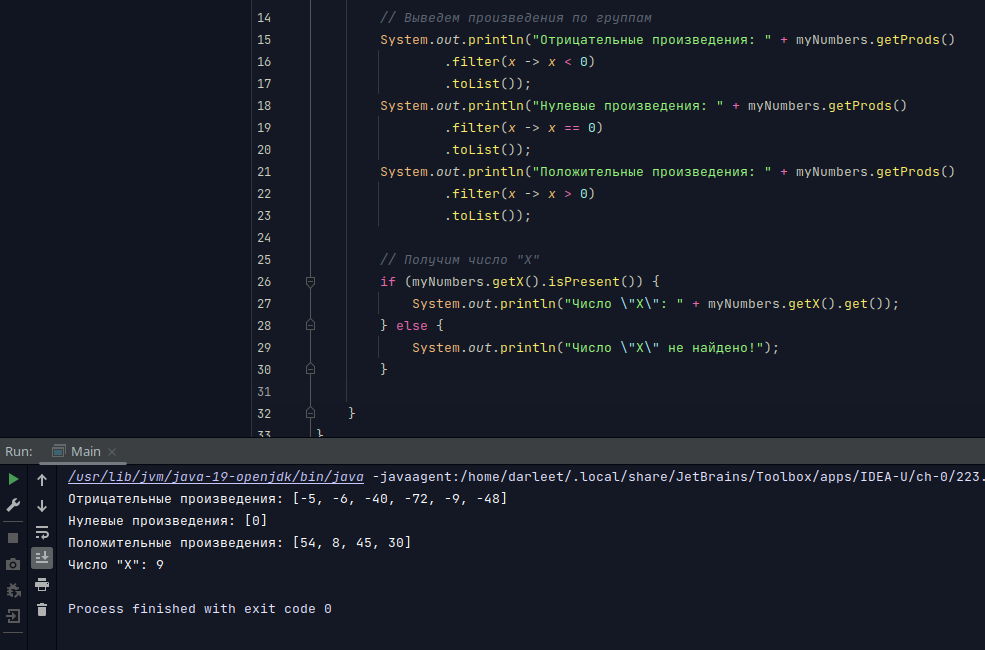
\includegraphics[scale=0.55]{class_main.png}} 
\caption{Вывод программы} 
\label{fig:image} 
\end{figure}

\end{document}
